\documentclass{article}

\usepackage{mathtools,amsfonts}
\usepackage{enumerate}
\usepackage{fullpage}
\usepackage{array}
\usepackage{fancyvrb}

\begin{document}
\thispagestyle{empty}

\begin{center}
  \textbf{\Large Beginner Test 2}
  % LEVEL is Senior, Intermediate or Beginner
  % NUMBER is the test number: 1, 2, etc.
  \\ \vspace{1em}
  \textbf{\large January Camp 2021}
  \\ \vspace{1em}
  \textbf{\large Time: 4 hours}
\end{center}

\vspace{24pt}

\begin{enumerate}[1.]


\item % Adapted from AIME
A hat has $3$ purple stickers and $7$ orange stickers inside. Another hat has $5$ purple stickers and $n$ orange stickers. One sticker is randomly taken from each hat. The probability that both stickers have the same colour is $0.6$. Find $n$.


\item % Tim
We all know that naughts and crosses is played on a $3\times 3$ grid, but what would happen if we tried it on a $4\times 4$ grid? Show this is a rigged game by finding a winning strategy for one of the players.\\
\textit{Note: the winning condition is to get 3 of your symbols adjacently along a row, column or diagonal.}


\item % Tim
Find $x$:
\begin{center}
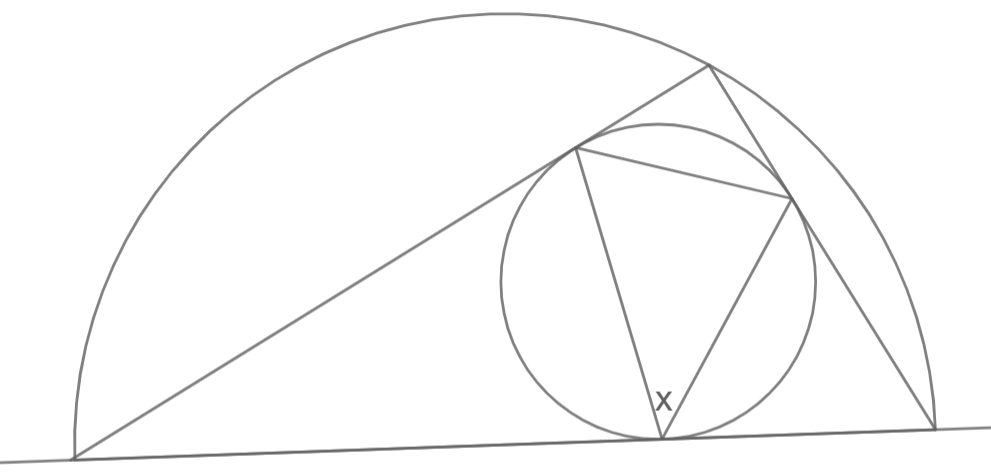
\includegraphics[scale=0.4]{angle_diagram.png}
\end{center}
\textit{Note: The outer arc is a semicircle.}


\item % Tim
You are given a ${k\times k}$ chessboard. You are told that there is a square on the chessboard where, if you place a queen, you will not be able to place a knight anywhere else such that both of them don't attack each other. Assuming this to be true, what is the maximum possible value of $k$?


\item % Tim
Find all pairs of positive integers $(n,k)$ satisfying $$n^3=(7k+3)^2$$


\item % Tim
There is a group of 6 people that are very suspicious of each other. It is very important to these people which of the rest of the group consider them to be friends. Now, because of the nature of this group, friendship is not a two way street! Person A may consider himself friends with Person B while Person B does not consider the same about Person A. A true friendship is a pair of people who both consider each other to be friends. If we are told that each of these 6 people considers exactly 3 others to be their friend, what is the maximum number of true friendships that can exist among these 6 people?


\item % Tim
Considering the sequences $a_n$ and $b_n$:
\begin{itemize}
\item $a_1=2$ and $b_1=3$
\item $a_{n+1}$ is obtained by taking the sum of the squares of the digits of $a_{n}$
\item $b_{n+1}$ is obtained by taking the sum of the squares of the digits of $b_n$
\end{itemize}
Find the maximum value of $gcd(a_k,b_k)$ for any integer $k\geq 1$, and find all $k$ where this maximum value occurs.\\
\textit{Note: gcd is greatest common divisor, which is the same as highest common factor.}


\item % British MO 2013/14 Round 1
In the acute-angled triangle $ABC$, the foot of the perpendicular from $B$ to $CA$ is $E$. Let $l$ be the tangent to the circumcircle of $\triangle ABC$ at $B$. The foot of the perpendicular from $C$ to $l$ is $F$. Prove that $EF$ is parallel to $AB$.


\item % Taariq
Let $x$ and $y$ be distinct real numbers such that $$x + 4 = (y - 2)^2 \quad\text{and}\quad y + 4 = (x - 2)^2$$
Find $x^2 + y^2$.

\item % Tim
\textbf{Bonus Question (from Advanced Test):}
A square-based pyramid has all of its edges the same length.
A cube is placed inside so that one of its faces lies on the base of the pyramid, and the opposite face has an edge along each side of the pyramid (think -- the natural way to put a cube in a pyramid).
Show that the sum of any of the cube's edge lengths with any of the cube's face diagonal lengths is the same as the edge length of the pyramid.


\end{enumerate}


\vfill
% ASCII art
\centering
\begin{BVerbatim}
>o)
(_>
\end{BVerbatim}

\end{document}